\section{Speaker Array: Measurement Results}
In order to investigate, how all the previous considerations about beamforming fare, when they are actually implemented, a series of measurements with a custom built speaker array has been conducted. A measurement protocol is given in \autoref{ax:directional_3}, as well as an overview over what individual measurements were conducted and what kinds of results were achieved. It is highly recommended to refer to the appendix when ambiguities occur while reading the following section.

\subsection{Beam Width}
As mentioned in \autoref{ch:intro}, for many practical applications it is desirable, that a sound sources radiates more sound into a particular direction then into other directions. Evenness over a given frequency range is often desirable. \autoref{fig:beamwidth_array} shows the measured relative pressure emission from the speaker array along the circumference of the speaker array in the frequency range of \SIrange{60}{300}{\hertz}. \autoref{fig:beamdwidth_array_off} shows the case, where all three speakers in the array play exactely the same signal, hence no beamforming is happening, wheras for \autoref{fig:beamdwidth_array_on}, beamforming was enabled. 
There is a significant difference in terms of directionality. Without beamforming, the sound emission from the array can be considered almost omnidirectional up to a frequency of approx. \SI{150}{\hertz}. At frequencies higher then this, an attenuation in the order of magnitude of \SIrange{3}{6}{\decibel} can be recorded near $\pm \SI{120}{\degree}$ in relation to the main axis of the array.
The picture drastically changes when beamforming is enabled. 
\begin{figure}[h]
	\centering
	\begin{subfigure}[c]{\textwidth}
		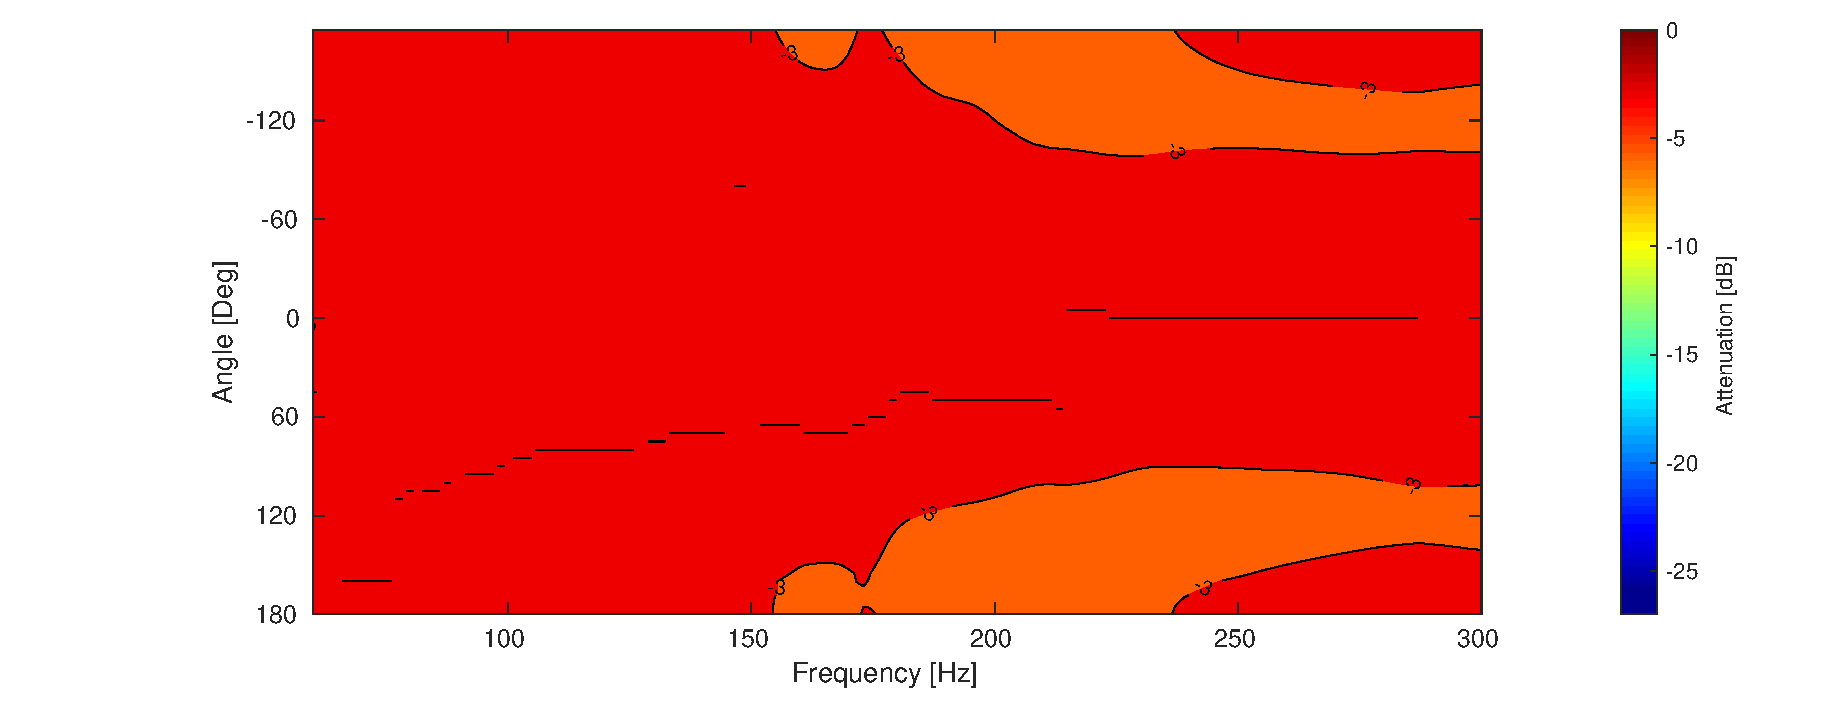
\includegraphics[width=1\textwidth]{beamwidth_disabled.eps}
		\subcaption{Speaker array, beamforming disabled.}
		\label{fig:beamdwidth_array_off}
	\end{subfigure}\\
		\begin{subfigure}[c]{\textwidth}
		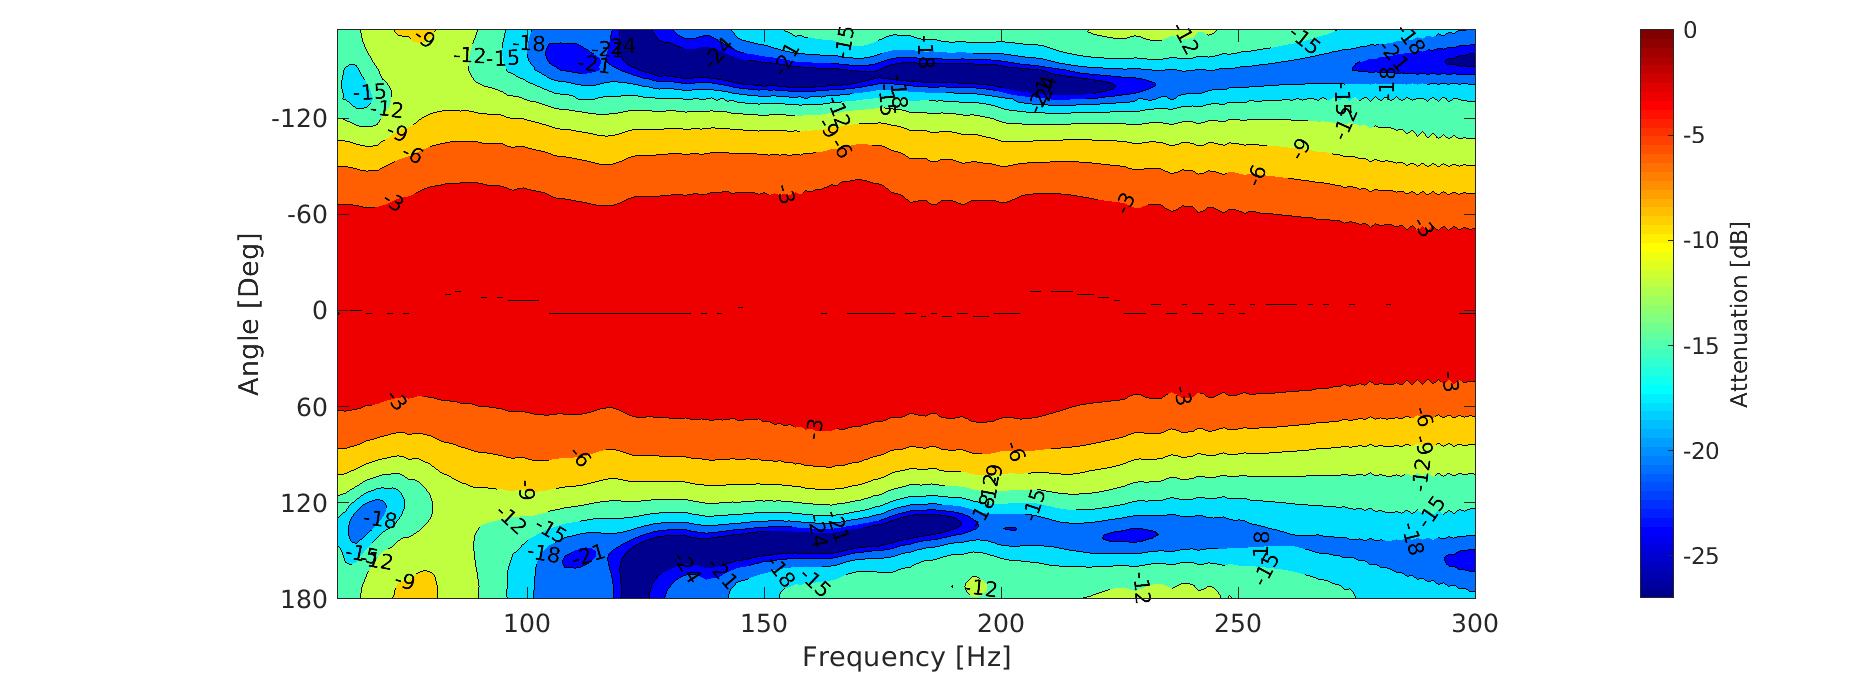
\includegraphics[width=1\textwidth]{beamwidth_final.eps}
		\subcaption{Speaker array, beamforming enabled.}
		\label{fig:beamdwidth_array_on}
	\end{subfigure}\\
	\caption{Contour plots of the relative level over frequency and angle, based on data from the measurements in \autoref{ax:directional_3}}
	\label{fig:beamwidth_array}
\end{figure}